%%%%%%%%%%%%%%%%%%%%%%%%%%%%%%%%%%%%%%%%%
% Arsclassica Article
% LaTeX Template
% Version 1.1 (1/8/17)
%
% This template has been downloaded from:
% http://www.LaTeXTemplates.com
%
% Original author:
% Lorenzo Pantieri (http://www.lorenzopantieri.net) with extensive modifications by:
% Vel (vel@latextemplates.com)
%
% License:
% CC BY-NC-SA 3.0 (http://creativecommons.org/licenses/by-nc-sa/3.0/)
%
%%%%%%%%%%%%%%%%%%%%%%%%%%%%%%%%%%%%%%%%%

%----------------------------------------------------------------------------------------
%	PACKAGES AND OTHER DOCUMENT CONFIGURATIONS
%----------------------------------------------------------------------------------------

\documentclass[
10pt, % Main document font size
a4paper, % Paper type, use 'letterpaper' for US Letter paper
oneside, % One page layout (no page indentation)
%twoside, % Two page layout (page indentation for binding and different headers)
headinclude,footinclude, % Extra spacing for the header and footer
BCOR5mm, % Binding correction
]{scrartcl}

%%%%%%%%%%%%%%%%%%%%%%%%%%%%%%%%%%%%%%%%%
% Arsclassica Article
% Structure Specification File
%
% This file has been downloaded from:
% http://www.LaTeXTemplates.com
%
% Original author:
% Lorenzo Pantieri (http://www.lorenzopantieri.net) with extensive modifications by:
% Vel (vel@latextemplates.com)
%
% License:
% CC BY-NC-SA 3.0 (http://creativecommons.org/licenses/by-nc-sa/3.0/)
%
%%%%%%%%%%%%%%%%%%%%%%%%%%%%%%%%%%%%%%%%%

%----------------------------------------------------------------------------------------
%	REQUIRED PACKAGES
%----------------------------------------------------------------------------------------

\usepackage[
nochapters, % Turn off chapters since this is an article        
beramono, % Use the Bera Mono font for monospaced text (\texttt)
eulermath,% Use the Euler font for mathematics
pdfspacing, % Makes use of pdftex’ letter spacing capabilities via the microtype package
dottedtoc % Dotted lines leading to the page numbers in the table of contents
]{classicthesis} % The layout is based on the Classic Thesis style

\usepackage{arsclassica} % Modifies the Classic Thesis package

\usepackage[T1]{fontenc} % Use 8-bit encoding that has 256 glyphs

\usepackage[utf8]{inputenc} % Required for including letters with accents

\usepackage{graphicx} % Required for including images
\graphicspath{{Figures/}} % Set the default folder for images

\usepackage{enumitem} % Required for manipulating the whitespace between and within lists

\usepackage{lipsum} % Used for inserting dummy 'Lorem ipsum' text into the template

\usepackage{subfig} % Required for creating figures with multiple parts (subfigures)

\usepackage{amsmath,amssymb,amsthm} % For including math equations, theorems, symbols, etc

\usepackage{varioref} % More descriptive referencing

%----------------------------------------------------------------------------------------
%	THEOREM STYLES
%---------------------------------------------------------------------------------------

\theoremstyle{definition} % Define theorem styles here based on the definition style (used for definitions and examples)
\newtheorem{definition}{Definition}

\theoremstyle{plain} % Define theorem styles here based on the plain style (used for theorems, lemmas, propositions)
\newtheorem{theorem}{Theorem}

\theoremstyle{remark} % Define theorem styles here based on the remark style (used for remarks and notes)

%----------------------------------------------------------------------------------------
%	HYPERLINKS
%---------------------------------------------------------------------------------------

\hypersetup{
%draft, % Uncomment to remove all links (useful for printing in black and white)
colorlinks=true, breaklinks=true, bookmarks=true,bookmarksnumbered,
urlcolor=webbrown, linkcolor=RoyalBlue, citecolor=webgreen, % Link colors
pdftitle={}, % PDF title
pdfauthor={\textcopyright}, % PDF Author
pdfsubject={}, % PDF Subject
pdfkeywords={}, % PDF Keywords
pdfcreator={pdfLaTeX}, % PDF Creator
pdfproducer={LaTeX with hyperref and ClassicThesis} % PDF producer
} % Include the structure.tex file which specified the document structure and layout

\hyphenation{Fortran hy-phen-ation} % Specify custom hyphenation points in words with dashes where you would like hyphenation to occur, or alternatively, don't put any dashes in a word to stop hyphenation altogether

%----------------------------------------------------------------------------------------
%	TITLE AND AUTHOR(S)
%----------------------------------------------------------------------------------------

\title{\normalfont\spacedallcaps{Artificial intelligence : project 1}} % The article title

%\subtitle{Subtitle} % Uncomment to display a subtitle

\subtitle{\spacedallcaps{DESIGNING OF SEARCH AGENTS USING PACMAN
}} % The article author(s) - author affiliations need to be specified in the AUTHOR AFFILIATIONS 
\author{\spacedallcaps{team: the holy trinity}}
%\suauthor{\spacedallcaps{members}}
\date{} % An optional date to appear under the author(s)

%----------------------------------------------------------------------------------------

\usepackage{mathtools}
\DeclarePairedDelimiter\ceil{\lceil}{\rceil}
\DeclarePairedDelimiter\floor{\lfloor}{\rfloor}

\usepackage{algorithm}
\usepackage{algorithmic}
\usepackage{graphicx}

\usepackage{epstopdf} %%package to overcome problem with eps in pdf files
\newcommand\tab[1][1cm]{\hspace*{#1}}
\begin{document}

%----------------------------------------------------------------------------------------
%	HEADERS
%----------------------------------------------------------------------------------------

\renewcommand{\sectionmark}[1]{\markright{\spacedlowsmallcaps{#1}}} % The header for all pages (oneside) or for even pages (twoside)
%\renewcommand{\subsectionmark}[1]{\markright{\thesubsection~#1}} % Uncomment when using the twoside option - this modifies the header on odd pages
\lehead{\mbox{\llap{\small\thepage\kern1em\color{halfgray} \vline}\color{halfgray}\hspace{0.5em}\rightmark\hfil}} % The header style

\pagestyle{scrheadings} % Enable the headers specified in this block

%----------------------------------------------------------------------------------------
%	TABLE OF CONTENTS & LISTS OF FIGURES AND TABLES
%----------------------------------------------------------------------------------------

\maketitle % Print the title/author/date block

\setcounter{tocdepth}{2} % Set the depth of the table of contents to show sections and subsections only

\tableofcontents % Print the table of contents

\listoffigures % Print the list of figures

\listoftables % Print the list of tables

\newpage % Start the article content on the second page, remove this if you have a longer abstract that goes onto the second page

%----------------------------------------------------------------------------------------
%	INTRODUCTION
%----------------------------------------------------------------------------------------

\section{{\textbf{Introduction}}}

In this project we are experimenting with 4 main search algorithms.
\begin{itemize}
    \item Depth First Search
    \item Breadth First Search
    \item Uniform Cost Search
    \item A* search
\end{itemize}
The Pacman AI projects were developed at UC Berkeley, primarily by
John DeNero and Dan Klein \cite{ref_UCB} for educational purposes. We will use python$3$ as out tool to code the search algorithms.
After that we will compare these 4 different search algorithms and compare them in terms of:
\begin{itemize}
    \item Performance
    \item Completeness
    \item Optimality
\end{itemize}





\section{\textbf{Depth First Search}}
\subsection*{\spacedallcaps{Problem Statement : Find a fixed food dot using depth first search algorithm}}
Depth First Search \cite{ref_russel} is an uninformed search strategy also called blind search strategy which means that the strategies have no additional information about the states other than the ones provided in the problem definition. It expands the deepest node in the current frontier of the search tree. It uses a stack to keep track of the generated nodes. As a stack follows LIFO principle, the last generated node is the first one chosen for expansion. Once a node is completely expanded, it is popped from the stack. The Depth First Search algorithm applied on pacman in small maze, medium maze and big maze are shown in Figure \ref{fig:fig_1_dfs_tinymaze}, Figure \ref{fig:fig_2_dfs_midmaze}, and Figure \ref{fig:fig_3_dfs_bigmaze.png}.

\subsection*{\spacedallcaps{ALGORITHM}}
\tab procedure DFS(G,v):\newline
\tab\tab let S be a stack\newline
\tab\tab S.push(v)\newline
\tab\tab while S is not empty\newline
\tab\tab\tab v = S.pop()\newline
\tab\tab\tab if v is not labeled as discovered:\newline
\tab\tab\tab\tab label v as discovered\newline
\tab\tab\tab\tab for all edges from v to w in G.adjacentEdges(v) do \newline
\tab\tab\tab\tab\tab S.push(w)\newline

\subsection*{\spacedallcaps{Complexity}}
The complexity of Depth First Search is : O($b^m$)\newline
where b is the branching factor and m is the maximum depth of the tree.\newline
The space complexity of Depth First Search is : O(bm)\newline
where b and m mean the same things as before.

\subsection*{\spacedallcaps{Complete}}
Depth First Search is complete if the tree is finite or else it is not complete(i.e, if the state space graph has cycles).

\subsection*{\spacedallcaps{optimal}}
Depth First Search is not optimal. It only finds the leftmost solution in the search tree regardless of the depth or cost of the node.


\begin{figure}[h!]
	\centering
	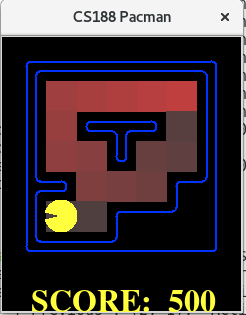
\includegraphics[width=0.20\textwidth]{images/fig_1_dfs_tinymaze.png}
	\caption{ DFS on tiny maze.}
	\label{fig:fig_1_dfs_tinymaze}
\end{figure}

\begin{figure}[h!]
	\centering
	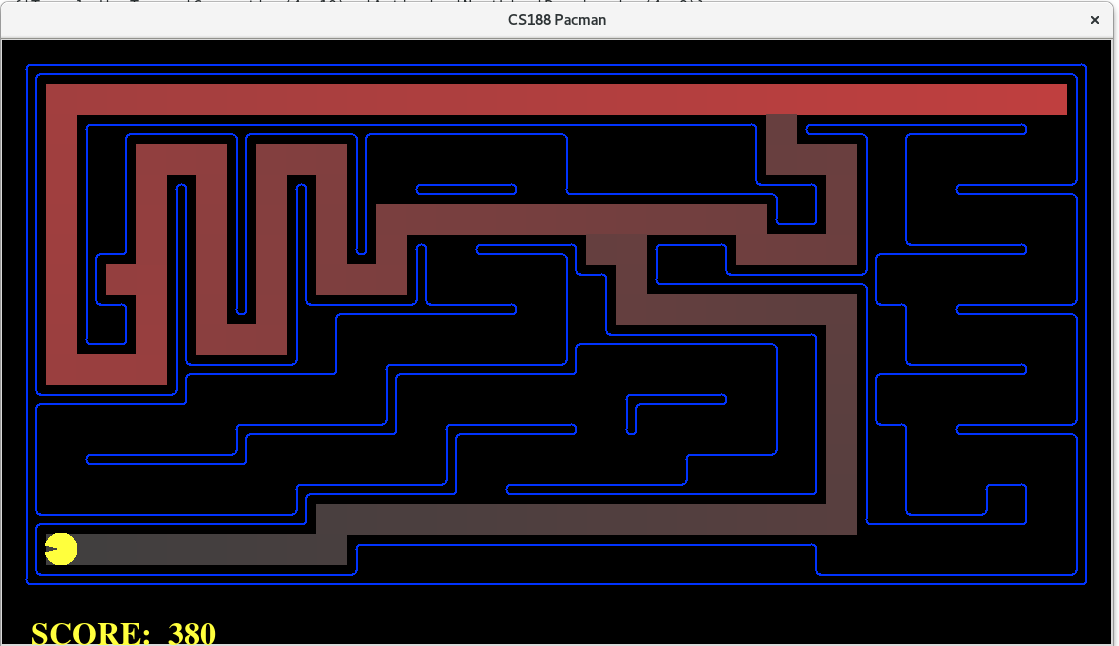
\includegraphics[width=.5\textwidth]{images/fig_2_dfs_midmaze.png}
	\caption{ DFS on medium maze.}
	\label{fig:fig_2_dfs_midmaze}
\end{figure}


\begin{figure}[h!]
	\centering
	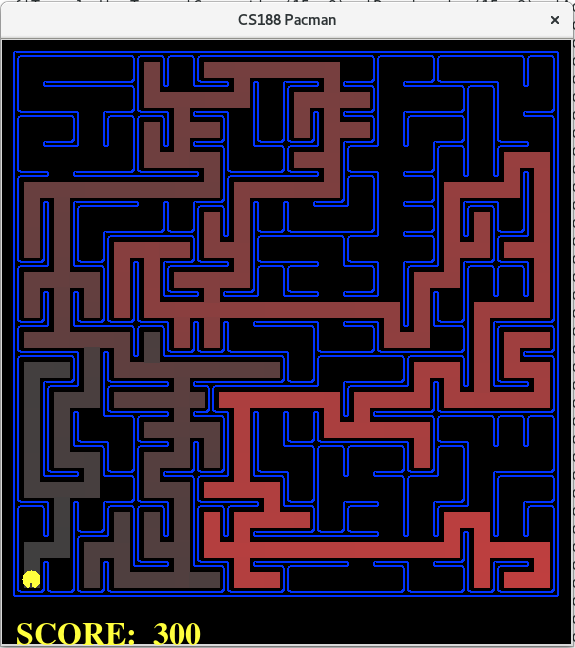
\includegraphics[width=.6\textwidth]{images/fig_3_dfs_bigmaze.png}
	\caption{ DFS on Big maze.}
	\label{fig:fig_3_dfs_bigmaze.png}
\end{figure}


%----------------------------------------------------------------------------------------------------------------------------
%                                                    Breadth First Search
%----------------------------------------------------------------------------------------------------------------------------
\section{{\textbf{Breadth First Search}}}
\subsection*{\spacedallcaps{Problem Statement : Find a fixed food dot using breadth first search algorithm}}
Breadth first search is a level by level search. All the nodes in a particular level are expanded before moving on to the next level. It expands the shallowest node first. It uses a queue data structure to maintain a list of all the nodes which have been expanded. The Breadth First Search algorithm applied on pacman in small maze, medium maze and big maze are shown in Figure \ref{fig:fig_4_bfs_tinymaze.png}, Figure \ref{fig:fig_5_bfs_mediumMaze}, and Figure \ref{fig:fig_6_bfs_bigmaze}.

\subsection*{\spacedallcaps{ALGORITHM}}
function BREADTH-FIRST-SEARCH(problem) returns a solution, or failure\newline\newline node $\leftarrow$ a node with STATE = problem.INITIAL-STATE, PATH-COST = 0\newline
if problem.GOAL-TEST(node.STATE) then return SOLUTION(node)\newline
frontier $\leftarrow$ a FIFO queue with node as the only element\newline
explored $\leftarrow$ an empty set\newline
loop do\newline
\tab if EMPTY?(frontier) then return failure\newline
\tab node $\leftarrow$ POP(frontier) /*chooses the shallowest node in the frontier*/\newline
\tab add node.STATE to explored\newline
\tab for each action in problem.ACTIONS(node.STATE) do\newline
\tab\tab child $\leftarrow$ CHILD-NODE(problem,node,action)\newline
\tab\tab if child.STATE is not in explored or frontier then\newline
\tab\tab\tab if problem.GOAL-TEST(child.STATE) then return SOLUTION(child)\newline
\tab\tab\tab frontier $\leftarrow$ INSERT (child,frontier)\newline

\subsection*{\spacedallcaps{Complexity}}
The time complexity of Breadth First Search is : O($b^d$)\newline where b is the branching factor of the search tree and d is the depth at which the shallowest goal node is situated.\newline The space complexity of Breadth First Search is : O($b^d$) i.e, it is dominated by the size of the frontier.

\subsection*{\spacedallcaps{Complete}}
Breadth First Search is complete because if a solution exits then the tree is finite.

\subsection*{\spacedallcaps{optimal}}
Breadth First Search is optimal only if the cost of all the arcs in the state space graph is the same.




\begin{figure}[h!]
	\centering
	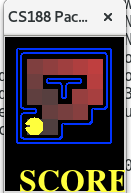
\includegraphics[width=0.20\textwidth]{images/fig_4_bfs_tinymaze.png}
	\caption{ BFS on tiny maze.}
	\label{fig:fig_4_bfs_tinymaze.png}
\end{figure}

\begin{figure}[h!]
	\centering
	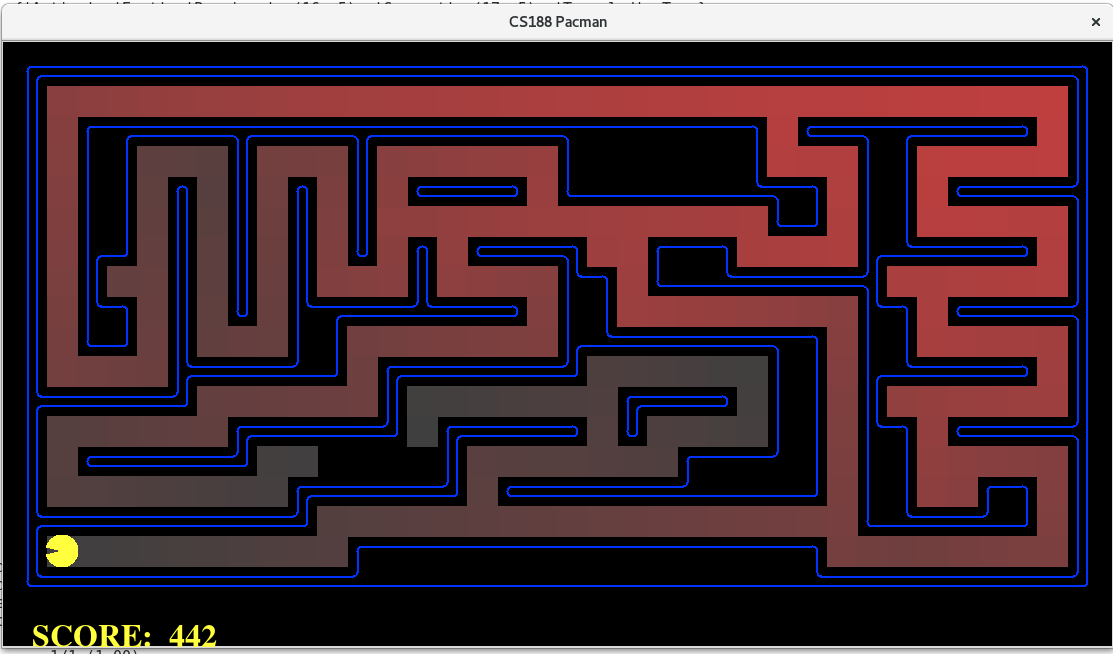
\includegraphics[width=.6\textwidth]{images/fig_5_bfs_mediumMaze.png}
	\caption{ BFS on medium maze.}
	\label{fig:fig_5_bfs_mediumMaze}
\end{figure}


\begin{figure}[h!]
	\centering
	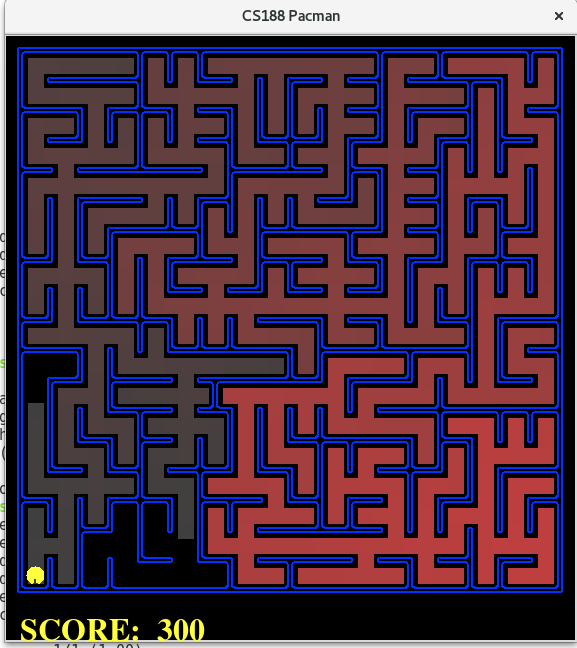
\includegraphics[width=.7\textwidth]{images/fig_6_bfs_bigmaze.png}
	\caption{ BFS on Big maze.}
	\label{fig:fig_6_bfs_bigmaze}
\end{figure}


%-----------------------------------------------------------------------------------------------------------------------------
%                                                   Uniform Cost Search
%-----------------------------------------------------------------------------------------------------------------------------

\section{\textbf{Uniform Cost Search}}
\subsection*{\spacedallcaps{Problem Statement : Find a fixed food dot by varying the cost function and using uniform cost search algorithm}}
Uniform Cost Search ,instead of expanding the shallowest node like Breadth First Search, expands the node n with the lowest cost path g(n). This is why the frontier is stored as a priority queue ordered by g. Uniform Cost Search applies the goal test to a node once it is selected for expansion rather than when it is first generated( as in the case of Breadth First Search and Depth First Search). This is because the first goal node that is generated may be on a sub-optimal path. It also includes a test to check whether a better goal state has been encountered. The Uniform Cost Search algorithm applied on pacman in small maze, medium maze and big maze are shown in Figure \ref{fig:fig_7_tiny_maze_ucs}, Figure \ref{fig:fig_8_medium_maze_ucs}, and Figure \ref{fig:fig_9_bigmaze_ucs}.

\subsection*{\spacedallcaps{ALGORITHM}}
function UNIFORM-COST-SEARCH(problem) returns a solution,or failure\newline
\tab node $\leftarrow$ a node with STATE = problem.INITIAL-STATE, PATH-COST = 0\newline
\tab frontier $\leftarrow$ a priority queue ordered by PATH-COST, with node as the only element\newline
\tab explored $\leftarrow$ an empty set\newline
\tab loop do\newline
\tab\tab if EMPTY?(frontier) then return failure\newline
\tab\tab node $\leftarrow$ POP(frontier) /*chooses the lowest-cost node in frontier */\newline
\tab\tab if problem.GOAL-TEST(node.STATE) then return SOLUTION(node)\newline
\tab\tab add node.STATE to explored\newline
\tab\tab for each action in problem.ACTIONS(node.STATE) do\newline
\tab\tab\tab child $\leftarrow$ CHILD-NODE(problem,node,action)\newline
\tab\tab\tab if child.STATE is not in explored or frontier then\newline
\tab\tab\tab\tab frontier $\leftarrow$ INSERT(child,frontier)\newline
\tab\tab\tab else if child.STATE is in frontier with higher PATH-COST then\newline
\tab\tab\tab\tab replace that frontier node with child\newline

\subsection*{\spacedallcaps{Complexity}}
Uniform-cost search is guided by path costs rather than depths, so its complexity is not
easily characterized in terms of b and d. Instead, let $c^*$
be the cost of the optimal solution, and assume that every action costs at least
$\epsilon$. Then the algorithm’s worst-case time and space
complexity is $O(b^{1+\floor{C^*/\epsilon}})$, which can be much greater than $b^d$.\newline
The space complexity of this algorithm is :  $O(b^{\floor{C^*/\epsilon}})$
\subsection*{\spacedallcaps{Complete}}
Uniform Cost Search is complete if the optimal solution has a finite cost and there are no arcs with negetive cost.
\subsection*{\spacedallcaps{optimal}}
Yes Uniform Cost Search is optimal.


\begin{figure}[h!]
	\centering
	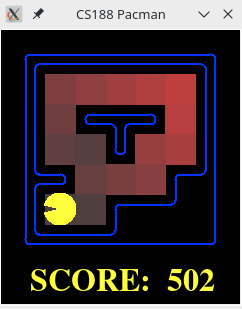
\includegraphics[width=0.20\textwidth]{images/fig_7_tiny_maze_ucs.png}
	\caption{ UCS on tiny maze.}
	\label{fig:fig_7_tiny_maze_ucs}
\end{figure}

\begin{figure}[h!]
	\centering
	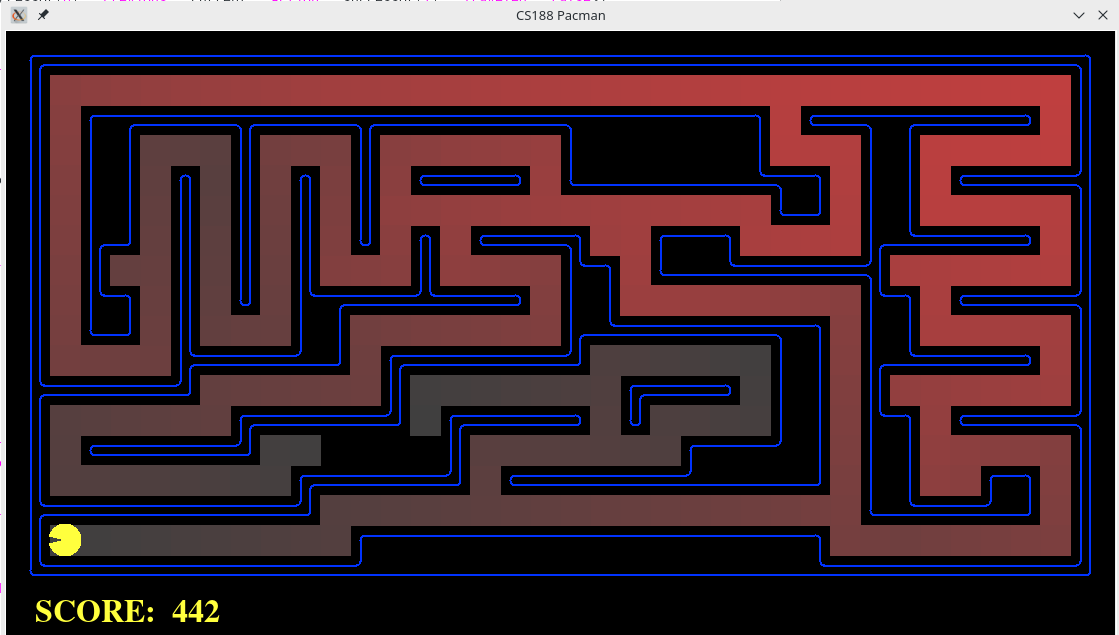
\includegraphics[width=.6\textwidth]{images/fig_8_medium_maze_ucs.png}
	\caption{ UCS on medium maze.}
	\label{fig:fig_8_medium_maze_ucs}
\end{figure}


\begin{figure}[h!]
	\centering
	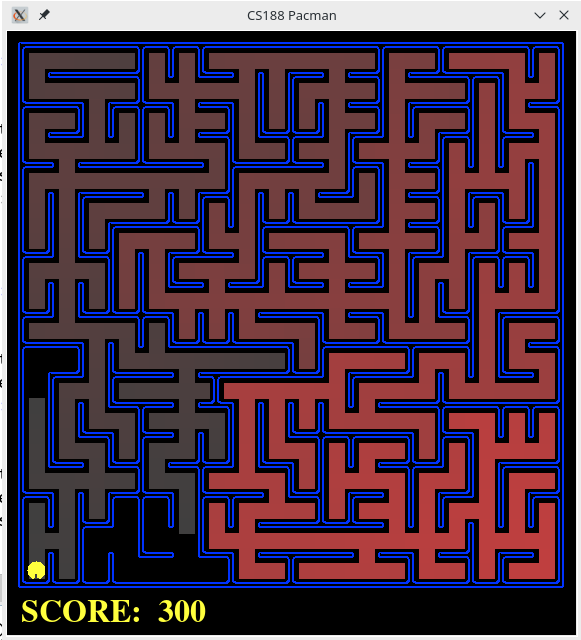
\includegraphics[width=.7\textwidth]{images/fig_9_bigmaze_ucs.png}
	\caption{ UCS on Big maze.}
	\label{fig:fig_9_bigmaze_ucs}
\end{figure}



%-----------------------------------------------------------------------------------------------------------------------------
%                                                        A* SEARCH
%-----------------------------------------------------------------------------------------------------------------------------
\section{{\textbf{A* Search}}}
\subsection*{\spacedallcaps{Problem Statement : Find a fixed food dot using A* search algorithm}}
A* search falls under the category of informed search strategy. This kind of search is also called best first search. A* search evaluates which node to combine using g(n) i.e, the cost to reach the node and h(n) i.e, the cost to get from the current node to the goal node, represented as :$$f(n)=g(n)+h(n)$$

The A* Search algorithm applied on pacman in small maze, medium maze and big maze are shown in Figure \ref{fig:fig_10_tinymaze_astar}, Figure \ref{fig:fig_11_mediummaze_astar}, and Figure \ref{fig:fig_12_bigmaze_astar}.

\subsection*{\spacedallcaps{ALGORITHM}}
function reconstruct\_path(cameFrom, current)\newline
\tab total\_path := {current}\newline
\tab while current in cameFrom.Keys:\newline
\tab\tab current := cameFrom[current]\newline
\tab\tab totalPath.prepend(current)\newline
\tab return totalPath\newline
function A\_Star(start, goal, h)\newline
openSet := {start}\newline
\tab cameFrom := an empty map\newline
\tab gScore := map with default value of Infinity\newline
\tab gScore[start] := 0\newline
\tab fScore := map with default value of Infinity\newline
\tab fScore[start] := h(start)\newline
\tab while openSet is not empty\newline
\tab\tab current := the node in openSet having the lowest fScore[] value\newline
\tab\tab if current = goal\newline
\tab\tab\tab return reconstruct\_path(cameFrom, current)\newline
\tab\tab openSet.Remove(current)\newline
\tab\tab closedSet.Add(current)\newline
\tab\tab for each neighbor of current\newline
\tab\tab\tab if neighbor in closedSet \newline
\tab\tab\tab\tab continue\newline
\tab\tab\tab tentative\_gScore := gScore[current] + d(current, neighbor)\newline
\tab\tab\tab if neighbor not in openSet\newline
\tab\tab\tab\tab openSet.add(neighbor)\newline
\tab\tab\tab if tentative\_gScore < gScore[neighbor]\newline
\tab\tab\tab\tab cameFrom[neighbor] := current\newline
\tab\tab\tab\tab gScore[neighbor] := tentative\_gScore\newline
\tab\tab\tab\tab fScore[neighbor] := gScore[neighbor] + h(neighbor)\newline
\tab return failure\newline

\subsection*{\spacedallcaps{Complexity}}
The time complexity of A* depends on the heuristic. In the worst case of an unbounded search space it will be : O($b^d$)\newline where b is the branching factor and d is the depth at which the solution resides in the tree.
The space complexity of A* is : O($b^d$)
\subsection*{\spacedallcaps{Complete}}
A* search is complete 
\subsection*{\spacedallcaps{optimal}}
A* search is optimal
%----------------------------------------------------------------------------------------
%	RESULTS AND DISCUSSION
%----------------------------------------------------------------------------------------



\begin{figure}[h!]
	\centering
	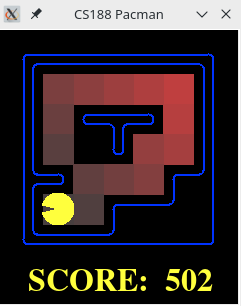
\includegraphics[width=0.20\textwidth]{images/fig_10_tinymaze_astar.png}
	\caption{ A-star on tiny maze.}
	\label{fig:fig_10_tinymaze_astar}
\end{figure}

\begin{figure}[h!]
	\centering
	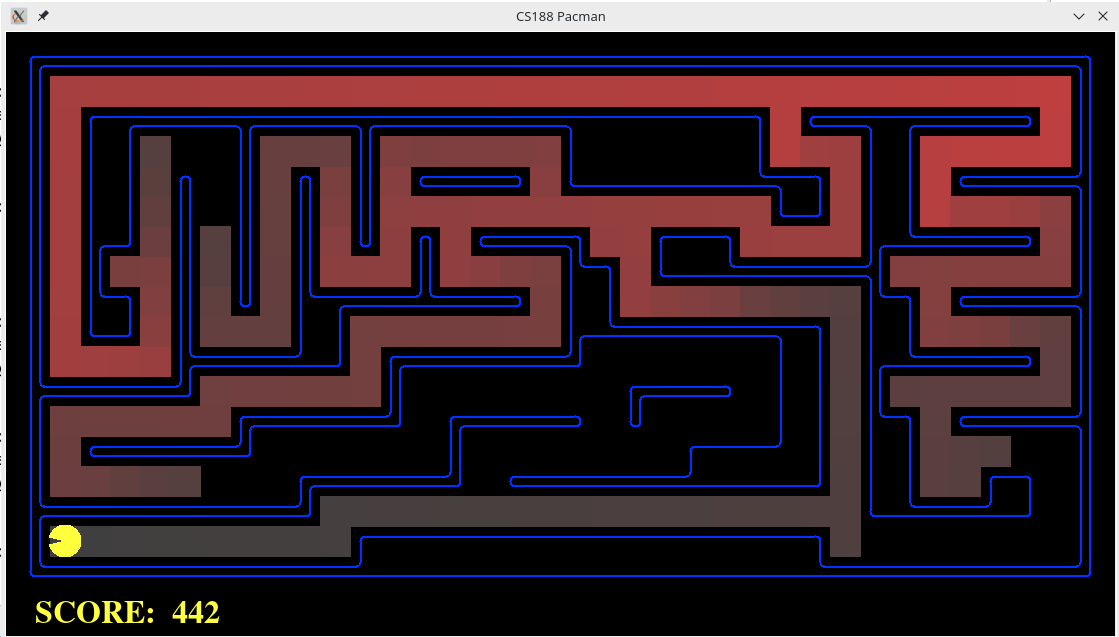
\includegraphics[width=.6\textwidth]{images/fig_11_mediummaze_astar.png}
	\caption{ A-star on medium maze.}
	\label{fig:fig_11_mediummaze_astar}
\end{figure}


\begin{figure}[h!]
	\centering
	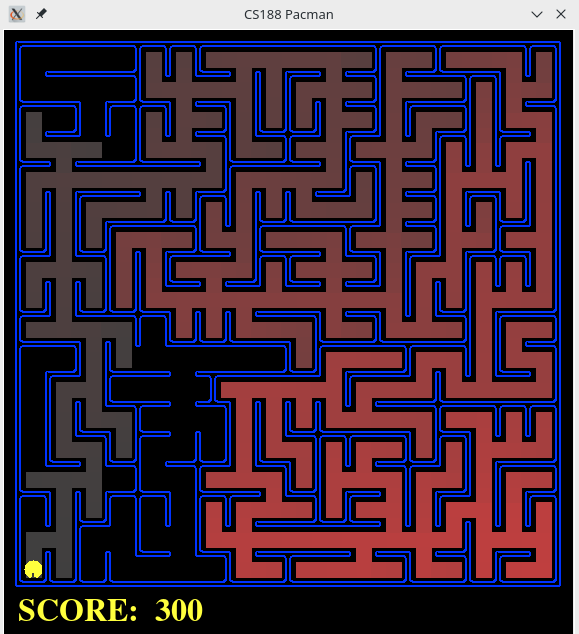
\includegraphics[width=.7\textwidth]{images/fig_12_bigmaze_astar.png}
	\caption{ A-star on Big maze.}
	\label{fig:fig_12_bigmaze_astar}
\end{figure}





\section{\textbf{Results and Discussion}}


We have worked with 3 uninformed search strategies and 1 informed search 
strategy. Obviously the informed search strategy worked better than the 
uninformed search strategies. Among the three uninformed search strategies 
Uniform Cost Search gives the best time complexity. But uniform cost search is 
useful only when the path costs are different otherwise it reduces to breadth 
first search.
If all the path costs are the same then breadth first search gives us the best 
time complexity of $O(b^d)$. But it has an exponential space complexity. Depth 
First Search gives us a linear space complexity but its time complexity is same 
as Breadth First Search. Furthermore DFS is neither complete nor optimal whereas
the other two are complete and optimal( given certain conditions).
The informed search strategy: A* search is optimal if we use admissible 
heuristics and consistent path cost( in case of graph search). But like BFS it 
has an exponential space complexity.
All the results obtained from the experiment are shown in \autoref{tab:res_table}.

% Please add the following required packages to your document preamble:
% \usepackage[table,xcdraw]{xcolor}
% If you use beamer only pass "xcolor=table" option, i.e. \documentclass[xcolor=table]{beamer}
% Please add the following required packages to your document preamble:
% \usepackage[table,xcdraw]{xcolor}
% If you use beamer only pass "xcolor=table" option, i.e. \documentclass[xcolor=table]{beamer}






\begin{thebibliography}{9}
	\bibitem{ref_UCB}
	The Pac-Man Projects, UC Berkeley CS188 Intro to AI -- Course Materials,
	available online at \href{http://ai.berkeley.edu/project_overview.html}{$http://ai.berkeley.edu/project_overview.html$}, last accessed on 27th August, 2019.
	
	\bibitem{ref_russel}
	 Russell, S., Norvig, P. (2010). Artificial Intelligence: A Modern Approach. Upper Saddle River, NJ: Prentice Hall.
	
	
\end{thebibliography}


	
\begin{table}[]
	\captionof{table}{Table of Results} \label{tab:res_table} 
	\resizebox{\columnwidth}{!}{
		\begin{tabular}{|c|ccc|r|}
			\hline
			\textbf{Search algorithm used}                                         & \textbf{Small Maze}                                                                   & \textbf{Medium Maze}                                                                                               & \textbf{Big Maze}                                                                        & \multicolumn{1}{c|}{\textbf{Description}}                                                                                             \\ \hline
			Depth First Search                                                     & \multicolumn{1}{c|}{\begin{tabular}[c]{@{}c@{}}10\\ \\ 15\\  \\ 500\\ \\ 500\\  \\ 1/1\\ \\ Win\end{tabular}} & \multicolumn{1}{c|}{\begin{tabular}[c]{@{}c@{}}130 \\ \\ 146\\  \\ 380\\  \\ 380\\  \\ 1/1\\  \\ Win\end{tabular}} & \begin{tabular}[c]{@{}c@{}}210\\ \\ 390\\ \\ 300\\ \\ 300\\ \\ 1/1\\ \\ Win\end{tabular} & \begin{tabular}[c]{@{}r@{}}Cost\\   \\ Search Node Expanded\\  \\ Average Score\\  \\ Scores\\  \\ Win Rate\\  \\ Record\end{tabular} \\ \hline
			Breadth First Search                                                   & \multicolumn{1}{c|}{\begin{tabular}[c]{@{}c@{}}8\\ \\ 15\\ \\ 502\\ \\ 502\\ \\ 1/1\\ \\ Win\end{tabular}}    & \multicolumn{1}{c|}{\begin{tabular}[c]{@{}c@{}}68\\ \\ 269\\ \\ 442\\ \\ 442\\ \\ 1/1\\ \\ Win\end{tabular}}       & \begin{tabular}[c]{@{}c@{}}210\\ \\ 620\\ \\ 300\\ \\ 300\\ \\ 1/1\\ \\ Win\end{tabular} & \begin{tabular}[c]{@{}r@{}}Cost\\   \\ Search Node Expanded\\  \\ Average Score\\  \\ Scores\\  \\ Win Rate\\  \\ Record\end{tabular} \\ \hline
			Uniform Cost Search                                                    & \multicolumn{1}{c|}{\begin{tabular}[c]{@{}c@{}}8\\ \\ 15\\ \\ 502\\ \\ 502\\ \\ 1/1\\ \\ Win\end{tabular}}    & \multicolumn{1}{c|}{\begin{tabular}[c]{@{}c@{}}68\\ \\ 269\\ \\ 442\\ \\ 442\\ \\ 1/1\\ \\ Win\end{tabular}}       & \begin{tabular}[c]{@{}c@{}}210\\ \\ 620\\ \\ 300\\ \\ 300\\ \\ 1/1\\ \\ Win\end{tabular} & \begin{tabular}[c]{@{}r@{}}Cost\\   \\ Search Node Expanded\\  \\ Average Score\\  \\ Scores\\  \\ Win Rate\\  \\ Record\end{tabular} \\ \hline
			\begin{tabular}[c]{@{}c@{}}A* using \\ Manhattan Distance\end{tabular} & \multicolumn{1}{c|}{\begin{tabular}[c]{@{}c@{}}8\\ \\ 14\\ \\ 502\\ \\ 502\\ \\ 1/1\\ \\ Win\end{tabular}}    & \multicolumn{1}{c|}{\begin{tabular}[c]{@{}c@{}}68\\ \\ 221\\ \\ 442\\ \\ 442\\ \\ 1/1\\ \\ Win\end{tabular}}        & \begin{tabular}[c]{@{}c@{}}210\\ \\ 549\\ \\ 300\\ \\ 300\\ \\ 1/1\\ \\ Win\end{tabular} & \begin{tabular}[c]{@{}r@{}}Cost\\   \\ Search Node Expanded\\  \\ Average Score\\  \\ Scores\\  \\ Win Rate\\  \\ Record\end{tabular} \\ \hline
		\end{tabular}
	}
\end{table}


\end{document}
